\documentclass[11pt,a4paper]{article}

% ── Packages ──────────────────────────────────────────────────────────────────
\usepackage[margin=1in]{geometry}
\usepackage[T1]{fontenc}
\usepackage{lmodern}
\usepackage{amsmath,amssymb}
\usepackage{graphicx}
\usepackage{array}
\usepackage[table]{xcolor}
\usepackage{booktabs}
\usepackage{tabularx}
\usepackage{caption}
\usepackage{titlesec}
\usepackage{parskip}
\usepackage{hyperref}
\usepackage{enumitem}
\usepackage{fancyhdr}
\usepackage{seqsplit}
\usepackage{tikz}
\usetikzlibrary{shapes.geometric,arrows.meta,positioning,fit,backgrounds,calc}

% ── Colours ───────────────────────────────────────────────────────────────────
\definecolor{titleblue}{RGB}{46,116,181}
\definecolor{darkblue}{RGB}{31,78,121}
\definecolor{rowgray}{RGB}{235,243,251}
\definecolor{headerblue}{RGB}{46,116,181}
\colorlet{ewublue}{darkblue}
\definecolor{nodeblue}{RGB}{224,231,255}
\definecolor{nodeindigo}{RGB}{199,210,254}
\definecolor{nodegreen}{RGB}{209,250,229}
\definecolor{nodegray}{RGB}{226,232,240}
\definecolor{codebg}{RGB}{238,242,255}

% ── Column types ──────────────────────────────────────────────────────────────
\newcolumntype{L}[1]{>{\raggedright\arraybackslash}p{#1}}
\newcolumntype{C}[1]{>{\centering\arraybackslash}p{#1}}

% ── Section formatting ────────────────────────────────────────────────────────
\titleformat{\section}{\large\bfseries\color{titleblue}}{\thesection\quad}{0em}{}
  [\color{titleblue}\titlerule]
\titleformat{\subsection}{\normalsize\bfseries\color{darkblue}}{\thesubsection\quad}{0em}{}
\titleformat{\subsubsection}{\small\bfseries\color{darkblue}}{\thesubsubsection\quad}{0em}{}
\titlespacing*{\section}{0pt}{18pt}{8pt}
\titlespacing*{\subsection}{0pt}{12pt}{4pt}

% ── Header / Footer ───────────────────────────────────────────────────────────
\pagestyle{fancy}
\fancyhf{}
\rhead{\small\color{gray}Software Design Document}
\lhead{\small\color{gray}scholar-agent}
\cfoot{\small\color{gray}\thepage}
\renewcommand{\headrulewidth}{0.4pt}

\hypersetup{colorlinks=true,linkcolor=titleblue,urlcolor=titleblue,citecolor=titleblue}

% ── Code / listing box ────────────────────────────────────────────────────────
\newcommand{\code}[1]{\leavevmode{\color{darkblue}\texttt{#1}}}
% break-friendly code for long identifiers inside narrow table cells
\newcommand{\bcode}[1]{\leavevmode{\color{darkblue}\texttt{\seqsplit{#1}}}}

% TikZ base styles
\tikzset{
  box/.style={rectangle,rounded corners=3pt,draw=darkblue!60,fill=nodeblue,
              text=black,align=center,inner sep=5pt,font=\footnotesize,minimum height=8mm},
  ibox/.style={box,fill=nodeindigo},
  gbox/.style={box,fill=nodegreen},
  store/.style={cylinder,shape border rotate=90,aspect=0.25,draw=darkblue!60,
                fill=nodegray,align=center,inner sep=4pt,font=\scriptsize,minimum height=11mm},
  actor/.style={circle,draw=darkblue!70,fill=white,align=center,font=\scriptsize,inner sep=3pt},
  fl/.style={-{Stealth[length=2.2mm]},draw=darkblue!70,font=\scriptsize},
  grp/.style={rectangle,rounded corners=4pt,draw=titleblue!40,fill=titleblue!5,inner sep=8pt},
}

\begin{document}

% ══════════════════════════════════════════════════════════════════════════════
% COVER PAGE
% ══════════════════════════════════════════════════════════════════════════════
\thispagestyle{empty}
\begin{center}
  
\includegraphics[width=3.2cm]{logo.jpg}\\[10pt]
  {\Large\bfseries\color{ewublue} EAST WEST UNIVERSITY}\\[3pt]
  {\normalsize\bfseries\color{ewublue} Department of Computer Science and Engineering}\\[5pt]
  {\large\bfseries\color{ewublue} SOFTWARE DESIGN DOCUMENT}\\[16pt]

  \fbox{%
    \parbox{0.85\textwidth}{%
      \centering\vspace{6pt}
      {\small\color{ewublue} Project Title}\\[6pt]
      {\large\bfseries scholar-agent: An Autonomous Scholarship and PhD\\
        Application Platform}\\[8pt]
      {\small\color{ewublue} Course: CSE 412 (Software Engineering)}\\[4pt]
    }%
  }
\end{center}

\vspace{16pt}
{\bfseries\color{ewublue} Submitted By}\\[6pt]
\renewcommand{\arraystretch}{1.4}
\begin{tabular}{|p{0.5\linewidth}|p{0.38\linewidth}|}
\hline
\rowcolor{ewublue!80}\textcolor{white}{\textbf{Student Name}} & \textcolor{white}{\textbf{Student ID}} \\
\hline
Md. Tamim Hasan Saykat       & 2022-1-60-289 \\ \hline
Md. Mahamudur Rahman Maharaz & 2022-3-60-182 \\ \hline
Naima Islam                  & 2022-3-60-215 \\ \hline
\end{tabular}

\vspace{14pt}


\vspace{16pt}
{\bfseries\color{ewublue} Submitted To}\\[6pt]
\noindent{\bfseries Yasin Sazid}\\
Lecturer
Department of Computer Science and Engineering, East West University

\vspace{10pt}
{\bfseries\color{ewublue} Design Methodology}\\[4pt]
\noindent Roger S. Pressman, \textit{Software Engineering: A Practitioner's Approach},
Chapter 13 (Architectural Design) and Chapter 14 (Component-Level Design).

\vfill
\begin{center}\small Department of Computer Science and Engineering\end{center}
\newpage

% ══════════════════════════════════════════════════════════════════════════════
\section{Introduction}

\subsection{Project Overview}
scholar-agent is a web platform for finding, tracking, and completing funded study
opportunities (scholarships and PhD positions) from a single account. It has two cooperating
parts. A \textbf{discovery engine} searches the live web, extracts structured opportunity
records, ranks them against the user's CV, and drafts application materials. A \textbf{system
of record}, which is the web application itself, stores accounts, tracks each application
through a status pipeline, manages professor outreach, and hosts a writing practice module.

The split between these two parts is deliberate. The discovery engine answers the question
\emph{``what opportunities exist?''} and writes to a shared knowledge base built from a graph
store and a vector store. The system of record answers \emph{``what is this user doing about
them?''} and writes to a per-user relational database. This separation is the central design
decision of the system, and the rest of the document refers back to it.

\subsection{List of Requirements}

\subsubsection{Functional Requirements}
\renewcommand{\arraystretch}{1.25}
\begin{tabularx}{\linewidth}{|C{1.35cm}|X|}
\hline
\rowcolor{headerblue}\textcolor{white}{\textbf{ID}} & \textcolor{white}{\textbf{Requirement}} \\
\hline
\mbox{FR-1} & A visitor can register and authenticate; all data is private to the account. \\
\rowcolor{rowgray}
\mbox{FR-2} & A user uploads or pastes a CV; the system extracts a structured profile. \\
\mbox{FR-3} & The system searches the web from free-text topics and extracts structured opportunity records. \\
\rowcolor{rowgray}
\mbox{FR-4} & Extracted opportunities are persisted to the knowledge base and de-duplicated by content identity. \\
\mbox{FR-5} & A user browses and filters the catalog and saves opportunities into a personal pipeline. \\
\rowcolor{rowgray}
\mbox{FR-6} & The system ranks opportunities against a profile and returns a score with a rationale. \\
\mbox{FR-7} & A user tracks each application through a status pipeline with a requirement checklist. \\
\rowcolor{rowgray}
\mbox{FR-8} & The system drafts a grounded cold email and Statement of Purpose per application, and persists them. \\
\mbox{FR-9} & A user maintains a professor-outreach record with a message thread and follow-up dates. \\
\rowcolor{rowgray}
\mbox{FR-10} & The system exports all deadlines and follow-ups as an importable calendar (.ics). \\
\mbox{FR-11} & A user keeps a watchlist of standing interests surfed automatically each day. \\
\rowcolor{rowgray}
\mbox{FR-12} & A user submits writing and receives criterion-level band scoring with feedback. \\
\hline
\end{tabularx}

\subsubsection{Non-Functional Requirements}
\begin{tabularx}{\linewidth}{|C{1.35cm}|L{2.7cm}|X|}
\hline
\rowcolor{headerblue}\textcolor{white}{\textbf{ID}} & \textcolor{white}{\textbf{Category}} & \textcolor{white}{\textbf{Requirement}} \\
\hline
\mbox{NFR-1} & Security & Passwords stored only as Argon2 hashes; sessions use signed JWTs; every query is scoped by \code{user\_id}. \\
\rowcolor{rowgray}
\mbox{NFR-2} & Portability & Runs with zero external services in development (SQLite, single provider); scales to Postgres and a multi-provider pool without code change. \\
\mbox{NFR-3} & Resilience & Inference degrades across a provider pool: on rate-limit or outage a call rolls to the next provider, and finally to a local model. \\
\rowcolor{rowgray}
\mbox{NFR-4} & Cost & Each research pass is bounded (paced request rate, capped page counts, per-role model routing) to fit free API tiers. \\
\mbox{NFR-5} & Maintainability & Build-free frontend; typed, layered backend with an automated test suite. \\
\rowcolor{rowgray}
\mbox{NFR-6} & Extensibility & New providers, agents, and API resources are added without modifying existing components (\S\ref{sec:principles}). \\
\hline
\end{tabularx}

\subsection{Technology Stack}
\begin{tabularx}{\linewidth}{|L{3.2cm}|L{4.5cm}|X|}
\hline
\rowcolor{headerblue}\textcolor{white}{\textbf{Layer}} & \textcolor{white}{\textbf{Technology}} & \textcolor{white}{\textbf{Role}} \\
\hline
Language & Python 3.12 & Backend and agents \\
\rowcolor{rowgray}
Web framework & FastAPI (ASGI) & HTTP API, dependency injection \\
Validation & Pydantic v2 & Domain schemas, request/response contracts \\
\rowcolor{rowgray}
ORM & SQLAlchemy 2.0 & Relational persistence \\
Relational DB & SQLite / PostgreSQL & System of record \\
\rowcolor{rowgray}
Graph store & Neo4j & Opportunity relationships \\
Vector store & Qdrant & Semantic search over opportunities \\
\rowcolor{rowgray}
Agent orchestration & LangGraph & Discovery state machine \\
Retrieval & fastembed (BGE + MiniLM) & Local embeddings and reranking \\
\rowcolor{rowgray}
Auth & passlib (Argon2), PyJWT & Hashing, token signing \\
Frontend & HTML + Alpine.js + Tailwind & Build-free reactive UI \\
\rowcolor{rowgray}
Model serving & Groq, Gemini, Ollama (pool) & LLM inference with failover \\
\hline
\end{tabularx}

% ══════════════════════════════════════════════════════════════════════════════
\section{Architectural Design}
This section follows Pressman Chapter 13: an architectural context diagram at two levels
(\S\ref{sec:acd}), a top-level component view (\S\ref{sec:comp}), and component
instantiation with elaboration (\S\ref{sec:elab}).

\subsection{Architectural Context Diagram}\label{sec:acd}
The architectural context diagram models how the system connects to entities outside its
boundary: superordinate systems that use it, subordinate systems it uses, and actors
(Pressman \S13.3.1).

\subsubsection{Level 0: System in Context}
At Level 0 the platform is one component. The student uses it; it depends on three external
subordinate systems: the web, the LLM provider pool, and the persistence stores.

\begin{center}
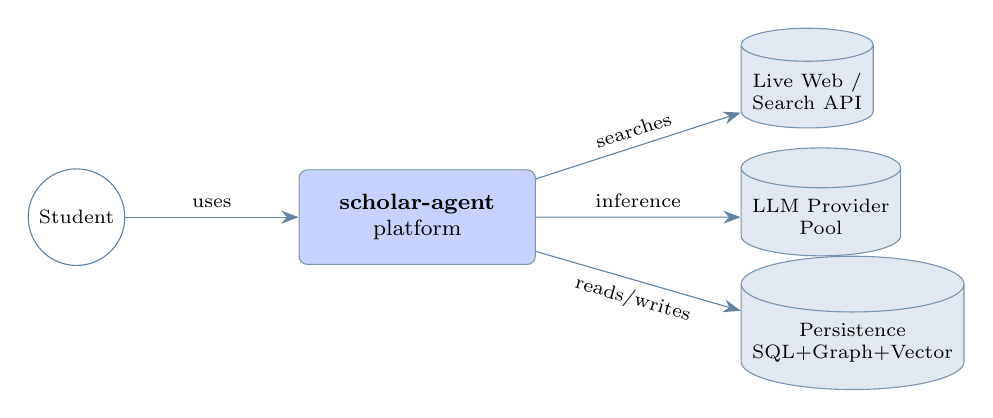
\begin{tikzpicture}[node distance=10mm]
  \node[actor] (stu) {Student};
  \node[ibox,right=22mm of stu,minimum width=30mm,minimum height=12mm] (sys)
    {\textbf{scholar-agent}\\platform};
  \node[store,right=26mm of sys,yshift=16mm] (web) {Live Web /\\Search API};
  \node[store,right=26mm of sys] (llm) {LLM Provider\\Pool};
  \node[store,right=26mm of sys,yshift=-16mm] (db) {Persistence\\SQL+Graph+Vector};
  \draw[fl] (stu) -- node[above]{uses} (sys);
  \draw[fl] (sys) -- node[above,sloped]{searches} (web);
  \draw[fl] (sys) -- node[above]{inference} (llm);
  \draw[fl] (sys) -- node[below,sloped]{reads/writes} (db);
\end{tikzpicture}
\end{center}

\subsubsection{Level 1: Internal Subsystems in Context}
At Level 1 the platform opens into its two subsystems and the shared knowledge base,
showing which external entities each subsystem contacts.

\begin{center}
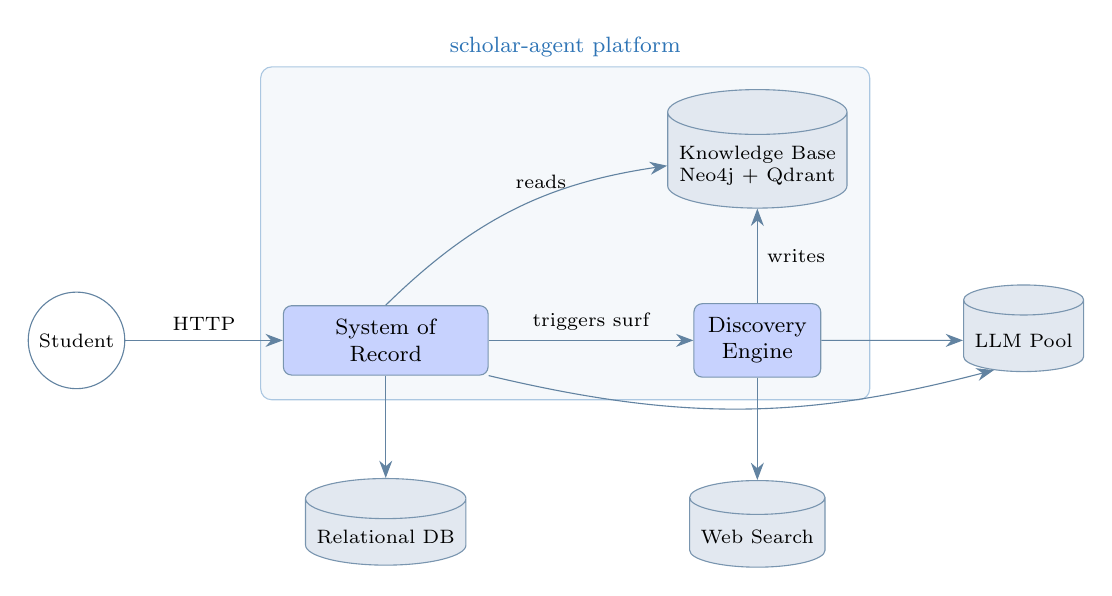
\begin{tikzpicture}[node distance=9mm]
  \node[actor] (stu) {Student};
  \node[ibox,right=20mm of stu,minimum width=26mm] (sor) {System of\\Record};
  \node[ibox,right=26mm of sor] (de) {Discovery\\Engine};
  \node[store,above=12mm of de] (kb) {Knowledge Base\\Neo4j + Qdrant};
  \node[store,below=13mm of sor] (sql) {Relational DB};
  \node[store,below=13mm of de] (web) {Web Search};
  \node[store,right=18mm of de] (llm) {LLM Pool};
  \begin{scope}[on background layer]
    \node[grp,fit=(sor)(de)(kb),label={[titleblue]above:\footnotesize scholar-agent platform}] {};
  \end{scope}
  \draw[fl] (stu) -- node[above]{HTTP} (sor);
  \draw[fl] (sor) -- node[above]{triggers surf} (de);
  \draw[fl] (de) -- node[right]{writes} (kb);
  \draw[fl] (sor.north) to[bend left=18] node[above,pos=0.6]{reads} (kb.west);
  \draw[fl] (sor) -- (sql);
  \draw[fl] (de) -- (web);
  \draw[fl] (de) -- (llm);
  \draw[fl] (sor.south east) to[bend right=14] (llm.south west);
\end{tikzpicture}
\end{center}

\noindent The System of Record is the only subsystem the student touches. It owns the
relational database and reads (never writes) the knowledge base. The Discovery Engine is
the only writer of the knowledge base and the only subsystem that reaches the outside web;
it is invoked by the System of Record, not the user. The knowledge base is the single
decoupling surface between the two.

\subsection{Top-Level Component Diagram}\label{sec:comp}
The macroscopic view decomposes the platform into components (Pressman \S13.4 to 13.5). Each
box is a package boundary in the codebase.

\begin{center}
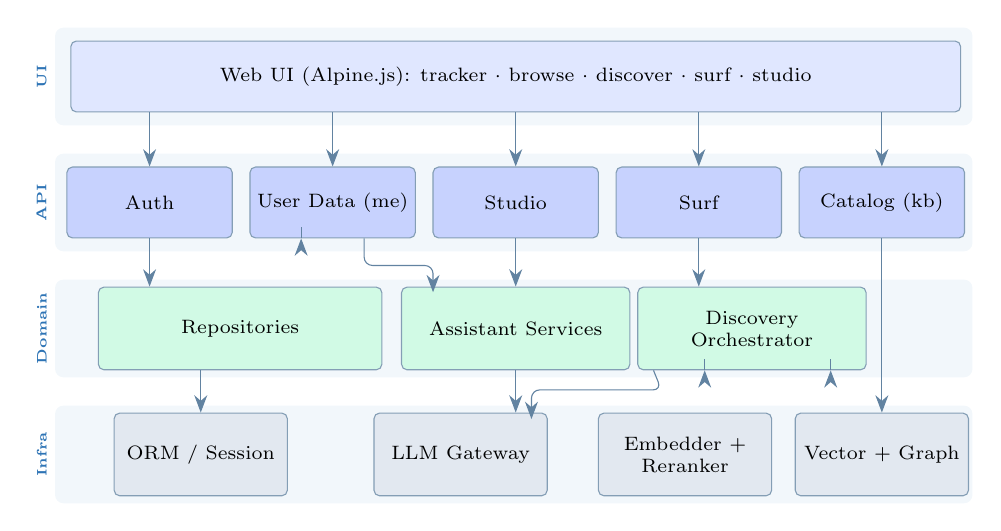
\begin{tikzpicture}[x=1cm,y=1cm]
  \tikzset{
    cbox/.style={rectangle,rounded corners=2pt,draw=darkblue!55,align=center,
                 font=\scriptsize,minimum width=2.35cm,minimum height=0.9cm,inner sep=2pt},
    ui/.style={cbox,fill=nodeblue,minimum width=11.4cm},
    api/.style={cbox,fill=nodeindigo},
    dom/.style={cbox,fill=nodegreen,minimum height=1.05cm},
    inf/.style={cbox,fill=nodegray,minimum height=1.05cm},
  }
  % ── horizontal layer bands (drawn first, behind everything) ──
  \begin{scope}[on background layer]
    \foreach \y/\name in {4.8/UI, 3.2/API, 1.6/Domain, 0.0/Infra}{
      \fill[titleblue!6,rounded corners=3pt] (0.55,\y-0.62) rectangle (12.2,\y+0.62);
      \node[titleblue,font=\tiny\bfseries,rotate=90] at (0.38,\y) {\name};
    }
  \end{scope}
  % ── Presentation: one bar spanning all five pages ──
  \node[ui,minimum width=11.3cm] (ui) at (6.4,4.8)
    {Web UI (Alpine.js): tracker $\cdot$ browse $\cdot$ discover $\cdot$ surf $\cdot$ studio};
  % ── API layer: five controllers on a uniform grid, ordered so each sits
  %    directly above the domain service it calls ──
  \node[api,minimum width=2.1cm] (auth)   at (1.75,3.2)  {Auth};
  \node[api,minimum width=2.1cm] (me)     at (4.075,3.2) {User Data (me)};
  \node[api,minimum width=2.1cm] (studio) at (6.4,3.2)   {Studio};
  \node[api,minimum width=2.1cm] (surf)   at (8.725,3.2) {Surf};
  \node[api,minimum width=2.1cm] (kbc)    at (11.05,3.2) {Catalog (kb)};
  % ── Domain layer: three services, each spanning its callers ──
  \node[dom,minimum width=3.6cm] (repo)   at (2.9,1.6)  {Repositories};
  \node[dom,minimum width=2.9cm] (assist) at (6.4,1.6)  {Assistant Services};
  \node[dom,minimum width=2.9cm] (orch)   at (9.4,1.6)  {Discovery\\Orchestrator};
  % ── Infrastructure layer: four adapters ──
  \node[inf,minimum width=2.2cm] (orm)   at (2.4,0.0)  {ORM / Session};
  \node[inf,minimum width=2.2cm] (llmgw) at (5.7,0.0)  {LLM Gateway};
  \node[inf,minimum width=2.2cm] (emb)   at (8.55,0.0) {Embedder +\\Reranker};
  \node[inf,minimum width=2.2cm] (vec)   at (11.05,0.0){Vector + Graph};
  % ── edges: pure vertical drops wherever a caller sits above its callee ──
  \foreach \t in {auth,me,studio,surf,kbc}{\draw[fl] (ui.south -| \t) -- (\t.north);}
  \draw[fl] (auth.south) -- (auth.south |- repo.north);
  \draw[fl] ($(me.south)+(-0.4,0)$) -- ($(me.south)+(-0.4,0)$ |- repo.north);
  \draw[fl] (studio.south) -- (studio.south |- assist.north);
  \draw[fl] (surf.south) -- (surf.south |- orch.north);
  \draw[fl] (kbc.south)  -- (kbc.south |- vec.north);        % catalog reads the KB directly
  \draw[fl] (repo.south -| orm.north) -- (orm.north);
  \draw[fl] (assist.south) -- (assist.south |- llmgw.north); % drafting/scoring inference
  \draw[fl] ($(orch.south)+(-0.6,0)$) -- ($(orch.south)+(-0.6,0)$ |- emb.north);
  \draw[fl] ($(orch.south)+(1.0,0)$)  -- ($(orch.south)+(1.0,0)$ |- vec.north);
  % two elbow routes (no crossings): me -> assistant, orchestrator -> gateway
  \draw[fl,rounded corners=3pt] ($(me.south)+(0.4,0)$) -- (4.475,2.4)
        -- (5.35,2.4) -- (5.35,2.06);
  \draw[fl,rounded corners=3pt] ($(orch.south)+(-1.25,0)$) -- (8.25,0.82)
        -- (6.6,0.82) -- (6.6,0.45);
\end{tikzpicture}
\end{center}

\subsection{Component Instantiation and Elaboration}\label{sec:elab}
Each component is given a responsibility and interface, then its operation is described.

\begin{description}[leftmargin=0pt,labelsep=6pt,style=nextline]
\item[Web UI.] Static HTML pages driven by small Alpine.js components. Each fetches JSON
with a bearer token from browser storage. No build step; Tailwind and Alpine load from a
CDN. The UI holds no business rules; it only renders state and issues requests.
\item[API Controllers.] FastAPI routers, one per resource family: \code{me} owns the user's
data (profile, applications, professors, watchlist, calendar, drafting), \code{kb} exposes
the read-only catalog, \code{surf} triggers discovery, \code{studio} scores writing. Every
controller depends on one \code{CurrentUser} dependency that decodes the JWT. This is the
single point where identity enters the system, which is what makes per-user isolation
enforceable (NFR-1).
\item[Domain / Services.] Repositories translate controller intent into ORM queries always
filtered by \code{user\_id}. The Discovery Orchestrator compiles and runs the agent state
machine. Assistant Services combine stored data with inference: drafting materials, building
the calendar, scoring writing.
\item[Infrastructure.] The LLM Gateway exposes one surface (\code{complete},
\code{structured}) over an ordered provider pool; on failure it rolls to the next provider,
finally to a local model (NFR-3). The Vector and Graph adapters wrap Qdrant and Neo4j. The
Embedder/Reranker produces vectors and re-scores candidates locally, so retrieval quality
does not depend on a paid API.
\end{description}

\subsubsection{Elaboration of the Discovery Orchestrator}
The orchestrator is the most behaviour-rich component. It is a LangGraph state machine over
a shared \code{PipelineState}. It has two entry paths, a deep web search and a fast database
lookup, that converge at matching and then enter a Scribe/Quality-Gate refinement loop.

\begin{center}
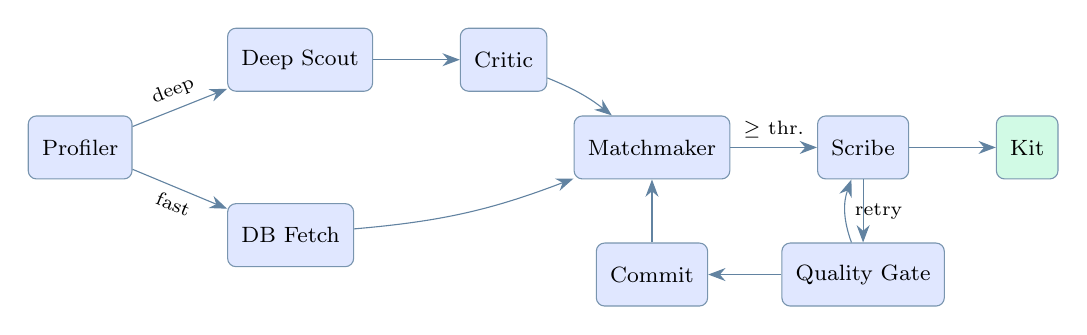
\begin{tikzpicture}[node distance=6mm and 11mm,every node/.style={font=\scriptsize}]
  \node[box] (prof) {Profiler};
  \node[box,above right=3mm and 12mm of prof] (scout) {Deep Scout};
  \node[box,below right=3mm and 12mm of prof] (dbf) {DB Fetch};
  \node[box,right=of scout] (crit) {Critic};
  \node[box,right=12mm of prof,xshift=44mm] (match) {Matchmaker};
  \node[box,right=of match] (scribe) {Scribe};
  \node[box,below=8mm of scribe] (qg) {Quality Gate};
  \node[box,below=8mm of match] (commit) {Commit};
  \node[gbox,right=of scribe] (kit) {Kit};
  \draw[fl] (prof) -- node[above,sloped]{deep} (scout);
  \draw[fl] (prof) -- node[below,sloped]{fast} (dbf);
  \draw[fl] (scout) -- (crit);
  \draw[fl] (crit) to[bend left=8] (match);
  \draw[fl] (dbf) to[bend right=8] (match);
  \draw[fl] (match) -- node[above]{$\geq$ thr.} (scribe);
  \draw[fl] (scribe) -- (qg);
  \draw[fl] (qg) to[bend left=20] node[right]{retry} (scribe);
  \draw[fl] (qg) -- (commit);
  \draw[fl] (commit) -- (match);
  \draw[fl] (scribe) -- (kit);
\end{tikzpicture}
\end{center}

\noindent The Profiler turns a CV into a structured profile and routes the run. The Deep
Scout searches the web and extracts opportunity records; the Critic fills missing deadlines.
The Matchmaker scores each opportunity against the profile and gates on a threshold. The
Scribe drafts materials; the Quality Gate verifies every claim is grounded in source text
and loops back until it passes. This bounded loop is what prevents hallucinated output.

% ══════════════════════════════════════════════════════════════════════════════
\section{Component-Level Design}
This section follows Pressman Chapter 14: the three class-elaboration steps
(\S\ref{sec:steps}), the derived class diagram (\S\ref{sec:class}), the design principles
(\S\ref{sec:principles}), and the database design (\S\ref{sec:db}).

\subsection{Elaboration of Design Components}\label{sec:steps}

\subsubsection{Step 1: Problem-Domain Design Classes}
These model the vocabulary of the problem itself and are technology-independent.

\begin{tabularx}{\linewidth}{|L{3.2cm}|X|}
\hline
\rowcolor{headerblue}\textcolor{white}{\textbf{Design class}} & \textcolor{white}{\textbf{Responsibility}} \\
\hline
\code{User} & Account holder; owns all other records. \\
\rowcolor{rowgray}
\code{StudentProfile} & Structured applicant record derived from a CV. \\
\code{Opportunity} & A funded position: title, institution, funding, deadline, supervisor. \\
\rowcolor{rowgray}
\code{SavedApplication} & A user's tracking record: status, checklist, drafted documents. \\
\code{ProfessorContact} & An outreach target with a message thread and follow-up schedule. \\
\rowcolor{rowgray}
\code{WatchlistItem} & A standing search interest surfed automatically. \\
\code{MatchResult} & Score and rationale relating a profile to an opportunity. \\
\rowcolor{rowgray}
\code{Artifact} (\code{ColdEmail}, \code{SOPDraft}) & A generated application document. \\
\code{WritingFeedback} & Criterion-level band scoring of a piece of writing. \\
\hline
\end{tabularx}

\subsubsection{Step 2: Infrastructure-Domain Design Classes}
These provide the technical services (persistence, network, security, mediation) the
problem-domain classes need.

\begin{tabularx}{\linewidth}{|L{3.4cm}|L{2.4cm}|X|}
\hline
\rowcolor{headerblue}\textcolor{white}{\textbf{Design class}} & \textcolor{white}{\textbf{Domain}} & \textcolor{white}{\textbf{Responsibility}} \\
\hline
\code{*Repository} & Persistence & Scoped CRUD, always filtered by \code{user\_id}. \\
\rowcolor{rowgray}
\code{Session} & Persistence & Unit-of-work / transaction boundary. \\
\code{VectorStore} & Persistence & Upsert and semantic search over opportunities. \\
\rowcolor{rowgray}
\code{GraphStore} & Persistence & Relationship storage and freshness pruning. \\
\code{Embedder/Reranker} & Compute & Local vector generation and re-scoring. \\
\rowcolor{rowgray}
\code{LLMClient} & Network & Provider-agnostic inference with failover. \\
\code{ProviderConfig} & Network & One endpoint's URL, key, per-role model map. \\
\rowcolor{rowgray}
\code{AuthService} & Security & Argon2 hashing, JWT issue/verify. \\
\code{CurrentUser} & Mediation & Resolves the authenticated user per request. \\
\hline
\end{tabularx}

\subsubsection{Step 3b: Component Interfaces}
Step 3b identifies the interface (message set) each component exposes. Defining them as
abstract contracts is what enables the substitution and inversion in \S\ref{sec:principles}.

\begin{tabularx}{\linewidth}{|L{3.35cm}|X|L{2.7cm}|}
\hline
\rowcolor{headerblue}\textcolor{white}{\textbf{Interface}} & \textcolor{white}{\textbf{Operations}} & \textcolor{white}{\textbf{Realised by}} \\
\hline
\code{InferenceProvider} & \code{complete}, \code{structured} & \code{LLMClient} over any \bcode{ProviderConfig} \\
\rowcolor{rowgray}
\code{Repository<T>} & \code{list}, \code{get}, \code{create}, \code{update}, \code{delete} & each concrete repository \\
\code{VectorIndex} & \code{upsert}, \code{hybrid\_search}, \code{scroll\_all}, \code{fetch\_by\_id} & Qdrant adapter \\
\rowcolor{rowgray}
\code{AgentNode} & \code{run(state)} $\to$ state & each of the six agents \\
\code{Assistant} & \code{draft\_application}, \code{draft\_email}, \code{build\_calendar}, \code{score\_writing} & Assistant services \\
\hline
\end{tabularx}

At the system boundary these interfaces surface as a REST API. The table below lists the
concrete endpoints each controller exposes, so the abstract interfaces above can be traced
to the running system.

\begin{tabularx}{\linewidth}{|L{2.5cm}|X|}
\hline
\rowcolor{headerblue}\textcolor{white}{\textbf{Resource}} & \textcolor{white}{\textbf{Endpoints}} \\
\hline
Auth & \code{POST /auth/signup} $\cdot$ \code{POST /auth/login} $\cdot$ \code{GET /auth/me} \\
\rowcolor{rowgray}
Profile & \code{GET /me/profile} $\cdot$ \code{PUT /me/profile} \\
Applications & \code{GET|POST /me/applications} $\cdot$ \code{GET|PATCH|DELETE /me/applications/\{id\}} $\cdot$ \code{POST /me/applications/\{id\}/draft} \\
\rowcolor{rowgray}
Professors & \code{GET|POST /me/professors} $\cdot$ \code{GET|PATCH|DELETE /me/professors/\{id\}} $\cdot$ \code{POST /me/professors/\{id\}/draft\_email} \\
Watchlist & \code{GET|POST /me/watchlist} $\cdot$ \code{DELETE /me/watchlist/\{id\}} \\
\rowcolor{rowgray}
Calendar & \code{GET /me/calendar.ics} (iCalendar export of deadlines and follow-ups) \\
Catalog & \code{GET /kb/opportunities} (read-only, deadline-sorted, expired excluded) \\
\rowcolor{rowgray}
Discovery & \code{POST /pipeline/stream} (SSE progress) $\cdot$ \code{POST /maintenance/surf} $\cdot$ \code{POST /maintenance/sweep} \\
Studio & \code{POST /studio/feedback} (band-scored writing assessment) \\
\hline
\end{tabularx}

\subsection{Class Diagram}\label{sec:class}
The classes below are derived directly from the Step 1 and Step 2 tables. Problem-domain
classes carry key attributes; infrastructure is shown through the Step 3b interfaces.

\begin{center}
\begin{tikzpicture}[x=1cm,y=1cm,font=\scriptsize]
  % UML class node: two compartments (name | attributes) separated by a rule
  \newcommand{\umlcls}[5]{% (id)(x,y)(fill)(name)(attrs)
    \node[rectangle,draw=darkblue!60,fill=#3,rounded corners=1pt,inner sep=0pt,
          minimum width=2.9cm,anchor=north] (#1) at #2 {%
      \begin{tabular}{@{}p{2.75cm}@{}}
        \centering\bfseries #4\tabularnewline[1pt]\hline\rule{0pt}{7pt}%
        \raggedright #5%
      \end{tabular}};
  }
  % ── problem domain. User sits in the middle so every ownership edge is a
  %    short, direct connection; Artifact sits under SavedApplication so the
  %    documents composition is a straight vertical. ──
  \umlcls{wl}{(0,7)}{nodeblue}{WatchlistItem}{+keyword\\+active}
  \umlcls{user}{(3.4,7)}{nodeblue}{User}{+id\\+email\\--password\_hash}
  \umlcls{app}{(6.8,7)}{nodeblue}{SavedApplication}{+opportunity\_ref\\+status\\+checklist\\+documents}
  \umlcls{opp}{(10.2,7)}{nodeblue}{Opportunity}{+title\\+funding\\+deadline}
  \umlcls{profc}{(0,4.4)}{nodeblue}{ProfessorContact}{+name\\+status\\+thread\\+linked\_app\_id}
  \umlcls{prof}{(3.4,4.4)}{nodeblue}{StudentProfile}{+full\_name\\+cv\_text\\+data}
  \umlcls{art}{(6.8,4.4)}{nodeblue}{Artifact}{+body}
  % ── Artifact subtypes fan in from below ──
  \umlcls{email}{(5.2,2.3)}{nodeblue}{ColdEmail}{+subject}
  \umlcls{sop}{(8.4,2.3)}{nodeblue}{SOPDraft}{+target}
  % ── infrastructure row ──
  \umlcls{llm}{(1.4,0.4)}{nodegreen}{\textit{«interface»} InferenceProvider}{+complete()\\+structured()}
  \umlcls{llmc}{(5.4,0.4)}{nodeblue}{LLMClient}{+pool : ProviderConfig[]}
  \umlcls{rep}{(9.4,0.4)}{nodegreen}{\textit{«interface»} Repository<T>}{+list() +get() +create()\\+update() +delete()}
  % ── relations ──
  % ownership (open diamond at the owner)
  \draw[{Diamond[open]}-] (user.west)  -- node[above]{1..*} (wl.east);
  \draw[{Diamond[open]}-] (user.east)  -- node[above]{1..*} (app.west);
  \draw[{Diamond[open]}-] (user.south) -- node[right,pos=.45]{1} (prof.north);
  \draw[{Diamond[open]}-] (user.south west) -- node[above,sloped,pos=.55]{1..*} (profc.north east);
  % dependency: application references a knowledge-base opportunity by id
  \draw[dashed,-{Stealth}] (app.east) -- node[above]{ref} (opp.west);
  % composition: an application owns its drafted documents
  \draw[{Diamond[open]}-] (art.north) -- node[right,pos=.45]{documents} (app.south);
  % generalisation (hollow triangle points at the parent)
  \draw[-{Triangle[open]}] (email.north) -- ($(art.south)+(-0.8,0)$);
  \draw[-{Triangle[open]}] (sop.north)   -- ($(art.south)+(0.8,0)$);
  % realisation: LLMClient realises InferenceProvider
  \draw[dashed,-{Triangle[open]}] (llmc.west) -- node[above,font=\tiny]{realises} (llm.east);
\end{tikzpicture}
\end{center}
\captionof{figure}{Design class diagram. Open diamonds mark aggregation/ownership; hollow
triangles mark generalisation and interface realisation; dashed arrows mark dependency.
\code{User} owns every per-user record; \code{Artifact} generalises the two generated
document types; \code{LLMClient} realises \code{InferenceProvider}.}

\subsection{Application of Pressman's Design Principles}\label{sec:principles}
Pressman (Ch. 14, ``Designing Class-Based Components'') prescribes the four SOLID
principles. Each is applied concretely below.

\begin{description}[leftmargin=0pt,style=nextline,labelsep=4pt]
\item[Open Closed Principle (OCP).] The \code{InferenceProvider} interface lets new
model back-ends be added without modifying callers. The provider pool is data-driven
(\code{providers.json}): adding Cerebras or a local model is a config entry, not a code
change. The agent pipeline is open for extension: a new \code{AgentNode} is registered on
the state graph while existing nodes stay closed. New API resources are new routers, not
edits to existing controllers.
\item[Liskov Substitution Principle (LSP).] Every \code{ProviderConfig} is substitutable
for every other behind \code{InferenceProvider}: the failover loop swaps a rate-limited Groq
provider for Gemini, then local Ollama, with no change to the contract the agents observe.
\code{ColdEmail} and \code{SOPDraft} are usable wherever an \code{Artifact} is expected, for
instance when appending to an application's \code{documents} list.
\item[Dependency Inversion Principle (DIP).] Policy does not depend on detail; both depend
on abstractions. The agents depend on the \code{InferenceProvider} and \code{VectorIndex}
interfaces, not on Groq's SDK or Qdrant's client. Controllers depend on repository
interfaces, not on SQLAlchemy internals. Concrete implementations are injected through
FastAPI's dependency system and cached factories, so source dependencies point toward
abstractions.
\item[Interface Segregation Principle (ISP).] Interfaces are narrow.
\code{InferenceProvider} exposes only \code{complete}/\code{structured};
\code{VectorIndex} exposes only retrieval; each repository exposes only its five CRUD
operations. A catalog-reading client depends on \code{VectorIndex} alone and is never forced
to know about the relational repositories. Controllers are split by resource family so none
carries operations its clients do not use.
\end{description}

\subsection{Database Design}\label{sec:db}
The relational schema is the system of record. Every user-owned table carries a
\code{user\_id} foreign key to \code{users} with cascade delete, so per-user isolation is
structural (NFR-1). Small bounded collections such as a checklist, a message thread, or a set
of drafted documents are stored as embedded JSON columns rather than child tables. They are
always fetched with their parent and never queried on their own, so a separate table would
add joins for no benefit.

\subsubsection{Entity Relationship (ER) Diagram}
\begin{center}
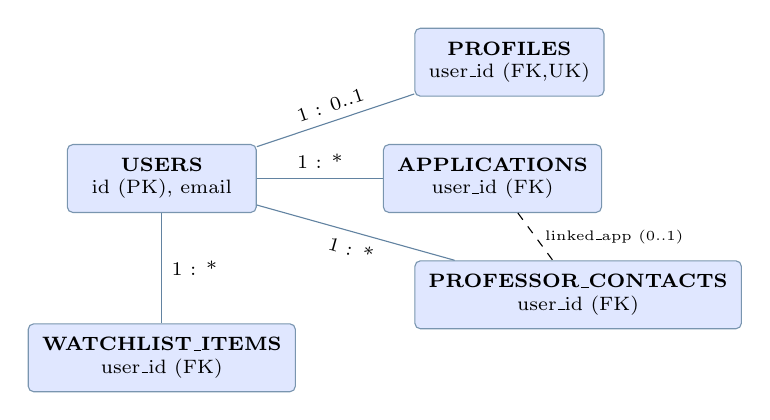
\begin{tikzpicture}[node distance=8mm and 16mm,every node/.style={font=\scriptsize}]
  \tikzset{ent/.style={rectangle,draw=darkblue!60,fill=nodeblue,align=center,
           rounded corners=2pt,inner sep=5pt,minimum width=24mm}}
  \node[ent] (u) {\textbf{USERS}\\\scriptsize id (PK), email};
  \node[ent,above right=6mm and 20mm of u] (p) {\textbf{PROFILES}\\\scriptsize user\_id (FK,UK)};
  \node[ent,right=of u] (a) {\textbf{APPLICATIONS}\\\scriptsize user\_id (FK)};
  \node[ent,below right=6mm and 20mm of u] (pc) {\textbf{PROFESSOR\_CONTACTS}\\\scriptsize user\_id (FK)};
  \node[ent,below=14mm of u] (w) {\textbf{WATCHLIST\_ITEMS}\\\scriptsize user\_id (FK)};
  \draw[fl,-] (u) -- node[above,sloped]{1 : 0..1} (p);
  \draw[fl,-] (u) -- node[above]{1 : *} (a);
  \draw[fl,-] (u) -- node[below,sloped]{1 : *} (pc);
  \draw[fl,-] (u) -- node[right]{1 : *} (w);
  \draw[dashed,-] (a) -- node[right,font=\tiny]{linked\_app (0..1)} (pc);
\end{tikzpicture}
\end{center}

\subsubsection{Table Schemas (key columns)}
\begin{tabularx}{\linewidth}{|L{3.4cm}|L{3.4cm}|X|}
\hline
\rowcolor{headerblue}\textcolor{white}{\textbf{Column}} & \textcolor{white}{\textbf{Type / Key}} & \textcolor{white}{\textbf{Notes}} \\
\hline
\rowcolor{titleblue!20}\multicolumn{3}{|l|}{\textbf{users}} \\
\hline
\code{id} & INTEGER PK & Identity root. \\
\code{email} & VARCHAR(320) UNIQUE & Login handle. \\
\code{password\_hash} & VARCHAR(255) & Argon2 hash only; the raw password is never stored. \\
\hline
\rowcolor{titleblue!20}\multicolumn{3}{|l|}{\textbf{profiles}} \\
\hline
\code{user\_id} & FK UNIQUE, CASCADE & One profile per user. \\
\code{data} & JSON & Structured \code{StudentProfile} extracted from the CV. \\
\hline
\rowcolor{titleblue!20}\multicolumn{3}{|l|}{\textbf{applications}} \\
\hline
\code{user\_id} & FK INDEX, CASCADE & Owner. \\
\code{opportunity\_ref} & VARCHAR(32) null & KB opportunity id, or null if added manually. \\
\code{status} & VARCHAR(40) INDEX & Pipeline stage: interested, preparing, applied, interview, offer, rejected, or waitlisted. \\
\code{checklist} & JSON & \code{[\{label, done\}]}. \\
\code{documents} & JSON & \code{[\{type,title,body,created\_at\}]}; server-generated drafts. \\
\hline
\rowcolor{titleblue!20}\multicolumn{3}{|l|}{\textbf{professor\_contacts}} \\
\hline
\code{status} & VARCHAR(40) INDEX & Outreach stage: to\_contact, emailed, replied, in\_conversation, meeting, or closed. \\
\bcode{linked\_application\_id} & INTEGER null & Soft link to an application. \\
\code{next\_followup\_at} & VARCHAR(32) null & Feeds the calendar export. \\
\code{thread} & JSON & \code{[\{direction,subject,body,at\}]}. \\
\hline
\rowcolor{titleblue!20}\multicolumn{3}{|l|}{\textbf{watchlist\_items}} \\
\hline
\code{keyword} & VARCHAR(300) & Standing search topic. \\
\code{last\_surfed\_at} & VARCHAR(32) null & Drives the oldest-first daily rotation. \\
\hline
\end{tabularx}

\subsubsection{Relationship Mappings}
\begin{itemize}[leftmargin=14pt,itemsep=2pt]
\item \textbf{users $\to$ profiles}: one-to-one (unique \code{user\_id}), cascade delete.
\item \textbf{users $\to$ applications / professor\_contacts / watchlist\_items}:
one-to-many with cascade delete, so removing an account removes all of its data.
\item \textbf{applications $\dashrightarrow$ professor\_contacts}: optional many-to-one soft
link (\code{linked\_application\_id}), not a hard FK, so outreach can exist independently.
\item \textbf{applications $\dashrightarrow$ knowledge base}: a cross-store reference by
content id (\code{opportunity\_ref}), deliberately not a FK, preserving the discovery/record
decoupling. The knowledge-base entities live in Neo4j/Qdrant, outside this relational model.
\end{itemize}

% ══════════════════════════════════════════════════════════════════════════════
\section{User Interface Design}
The interface is a small set of single-purpose pages sharing one top navigation bar and a
dark, glass-panel theme. The wireframes below are low-fidelity (boxes and labels only), so
they show layout and interaction without committing to final visual styling. Each screen is
shown separately.

% wireframe primitives
\tikzset{
  wframe/.style={rectangle,draw=darkblue!45,fill=white,line width=0.4pt},
  wbar/.style={rectangle,draw=darkblue!35,fill=nodeindigo!70,font=\tiny,inner sep=2pt,align=center},
  wfield/.style={rectangle,draw=darkblue!35,fill=gray!8,font=\tiny,inner sep=2pt,align=left},
  wbtn/.style={rectangle,rounded corners=2pt,draw=darkblue!50,fill=titleblue!25,font=\tiny,inner sep=2pt,align=center},
  wchip/.style={rectangle,rounded corners=3pt,draw=darkblue!30,fill=nodeblue,font=\tiny,inner sep=1.6pt},
  wcard/.style={rectangle,rounded corners=2pt,draw=darkblue!30,fill=gray!5,font=\tiny,align=left,inner sep=2.5pt},
  wlab/.style={font=\tiny,gray},
}

\subsection{Wireframe 1: Application Tracker (home)}
The home screen is a Kanban board with one column per pipeline stage. A fixed top bar carries
the brand, page navigation, a calendar-export action, and the account menu. Cards are dragged
between columns to change status.

\begin{center}
\begin{tikzpicture}[x=1cm,y=1cm]
  \draw[wframe] (0,0) rectangle (12,6.4);
  % top bar
  \node[wbar,minimum width=11.6cm,minimum height=0.5cm,anchor=north west] at (0.2,6.2)
    {};
  \node[font=\tiny\bfseries,anchor=west] at (0.35,5.95) {scholar$\cdot$agent};
  \foreach \i/\t in {0/Tracker,1/Browse,2/Discover,3/Build KB,4/Studio}{
    \node[font=\tiny,anchor=west] at (2.5+\i*1.35,5.95) {\t};}
  \node[wbtn,anchor=east] at (10.8,5.95) {Calendar};
  \node[font=\tiny,anchor=east] at (11.8,5.95) {user\,$\vee$};
  % column headers + cards
  \foreach \i/\h in {0/Interested,1/Preparing,2/Applied,3/Interview}{
    \node[wbar,minimum width=2.6cm,minimum height=0.4cm,anchor=north west] at (0.25+\i*2.9,5.4) {\h};}
  % a few cards
  \node[wcard,minimum width=2.5cm,minimum height=0.85cm,anchor=north west] at (0.3,4.85)
    {\textbf{DAAD PhD}\\TU Munich\\{\color{red!70}$\odot$ soon}};
  \node[wcard,minimum width=2.5cm,minimum height=0.85cm,anchor=north west] at (0.3,3.85)
    {\textbf{Chevening}\\UK};
  \node[wcard,minimum width=2.5cm,minimum height=0.85cm,anchor=north west] at (3.2,4.85)
    {\textbf{Erasmus MSc}\\$\odot$ Nov 1};
  \node[wcard,minimum width=2.5cm,minimum height=0.85cm,anchor=north west] at (6.1,4.85)
    {\textbf{Fulbright}\\applied};
  \node[wbtn,anchor=north east] at (11.75,5.4) {+ Add manually};
  \node[wlab,anchor=south west] at (0.25,0.1) {Drag a card between columns to change its status.};
\end{tikzpicture}
\end{center}

\subsection{Wireframe 2: Application Detail Drawer}
Clicking a card slides in a right-hand drawer (an in-place sub-state, not a new page). It
holds the status and deadline controls, a requirement checklist, a \emph{Materials} section
whose ``Draft email + SOP'' button generates and persists documents, and a notes field.

\begin{center}
\begin{tikzpicture}[x=1cm,y=1cm]
  \draw[wframe] (0,0) rectangle (12,5.6);
  \fill[gray!4] (0,0) rectangle (7.4,5.6);
  \node[wlab] at (3.7,2.8) {(tracker board behind, dimmed)};
  % drawer
  \draw[wframe,fill=gray!2] (7.4,0) rectangle (12,5.6);
  \node[font=\tiny\bfseries,anchor=north west] at (7.55,5.45) {DAAD PhD, TU Munich};
  \node[font=\tiny,anchor=north east] at (11.85,5.45) {$\times$};
  \node[wfield,minimum width=2.1cm,anchor=north west] at (7.55,4.85) {Status: Preparing $\vee$};
  \node[wfield,minimum width=2.0cm,anchor=north west] at (9.75,4.85) {Deadline: 2026-11-01};
  \node[font=\tiny\bfseries,anchor=north west] at (7.55,4.35) {Checklist};
  \foreach \i/\c/\t in {0/$\boxtimes$/CV,1/$\square$/SOP,2/$\square$/IELTS}{
    \node[font=\tiny,anchor=north west] at (7.55+\i*1.3,4.05) {\c\ \t};}
  \node[font=\tiny\bfseries,anchor=north west] at (7.55,3.5) {Materials};
  \node[wbtn,anchor=north east] at (11.85,3.55) {Draft email + SOP};
  \node[wcard,minimum width=4.2cm,anchor=north west] at (7.55,3.1) {$\triangleright$ PhD inquiry (Email)\quad copy $\cdot$ download};
  \node[wcard,minimum width=4.2cm,anchor=north west] at (7.55,2.55) {$\triangleright$ Statement of Purpose (SOP)};
  \node[wfield,minimum width=4.2cm,minimum height=0.8cm,anchor=north west] at (7.55,1.95) {Notes\ldots};
  \node[wbtn,anchor=south west] at (7.55,0.15) {Save changes};
  \node[font=\tiny,anchor=south east] at (11.85,0.15) {Cancel};
\end{tikzpicture}
\end{center}

\subsection{Wireframe 3: Browse Catalog and Writing Studio}
Two further screens are shown together. Browse is a filtered card grid over the knowledge
base; the Studio is a two-panel practice screen (input left, scored feedback right).

\begin{center}
\begin{tikzpicture}[x=1cm,y=1cm]
  % --- Browse ---
  \draw[wframe] (0,0) rectangle (5.7,5.4);
  \node[font=\tiny\bfseries,anchor=north west] at (0.15,5.3) {Browse};
  \node[wfield,minimum width=5.3cm,anchor=north west] at (0.2,4.9) {search title / university\ldots};
  \foreach \i/\t in {0/Scholarships,1/PhD,2/Fellowship}{
    \node[wchip,anchor=north west] at (0.2+\i*1.55,4.35) {\t};}
  \node[wchip,anchor=north west,fill=nodegreen] at (4.15,4.35) {Funded};
  \foreach \r in {0,1}{\foreach \c in {0,1,2}{
    \node[wcard,minimum width=1.6cm,minimum height=1.1cm,anchor=north west]
      at (0.2+\c*1.78,3.85-\r*1.35) {\textbf{Title}\\Univ.\\$\odot$ date\\{\color{titleblue}Save}};}}
  \node[wlab,anchor=south west] at (0.2,0.1) {3-col grid (1-col on mobile)};
  % --- Studio ---
  \draw[wframe] (6.3,0) rectangle (12,5.4);
  \node[font=\tiny\bfseries,anchor=north west] at (6.45,5.3) {Writing Studio};
  % left input
  \foreach \i/\t in {0/{IELTS T2},1/{T1},2/SOP,3/Acad.}{
    \node[wchip,anchor=north west] at (6.45+\i*0.9,4.85) {\t};}
  \node[wfield,minimum width=2.5cm,minimum height=0.5cm,anchor=north west] at (6.45,4.3) {task prompt\ldots};
  \node[wfield,minimum width=2.5cm,minimum height=1.6cm,anchor=north west] at (6.45,3.7) {your essay\ldots\\\\{\color{gray}142 words}};
  \node[wbtn,anchor=north west] at (6.45,1.95) {Assess};
  % right feedback
  \node[circle,draw=titleblue,fill=nodegreen,minimum size=0.9cm,font=\tiny,anchor=north west] at (9.3,4.85) {6.5};
  \node[wlab,anchor=north west] at (10.35,4.75) {overall band};
  \foreach \i/\t/\sc in {0/Task/6.0, 1/Coherence/6.5, 2/Lexis/6.5, 3/Grammar/7.0}{
    \node[wcard,minimum width=2.3cm,anchor=north west] at (9.3,4.0-\i*0.42) {\t\hfill {\color{titleblue}\sc}};}
  \node[wcard,minimum width=2.5cm,anchor=north west] at (9.3,2.1) {$\checkmark$ strengths / $\blacktriangle$ fixes};
\end{tikzpicture}
\end{center}

\subsection{Navigation Flow}
Authentication is the single entry gate: every other screen needs a valid session and
otherwise redirects to sign-in. The Tracker is the hub: the feature pages branch off it and
most actions return to it. The drawers are sub-states of the Tracker, so the flow stays
shallow.

\begin{center}
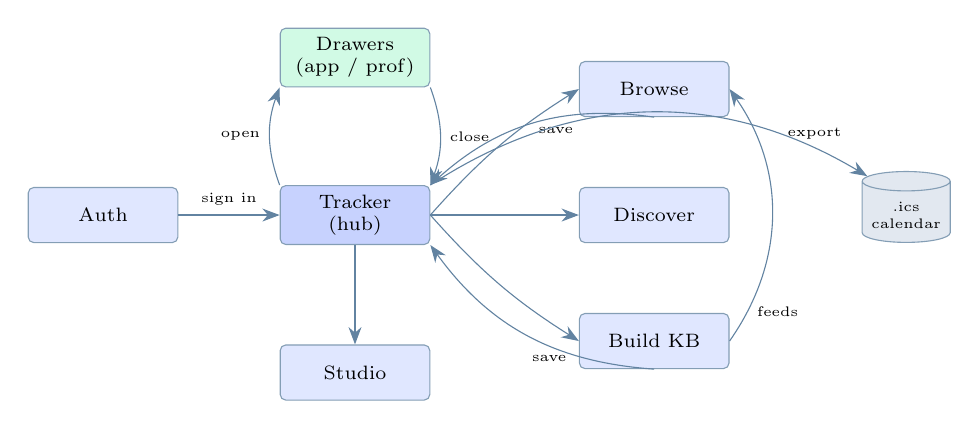
\begin{tikzpicture}[x=1cm,y=1cm,font=\scriptsize]
  \tikzset{nn/.style={rectangle,rounded corners=2pt,draw=darkblue!55,fill=nodeblue,
           minimum width=1.9cm,minimum height=0.7cm,align=center,font=\scriptsize},
           hub/.style={nn,fill=nodeindigo},
           sub/.style={nn,fill=nodegreen},
           st/.style={cylinder,shape border rotate=90,aspect=0.22,draw=darkblue!55,
                      fill=nodegray,font=\tiny,minimum height=0.9cm,align=center}}
  \node[nn] (auth) at (0,2) {Auth};
  \node[hub] (track) at (3.2,2) {Tracker\\(hub)};
  \node[sub] (draw) at (3.2,4) {Drawers\\(app / prof)};
  \node[nn] (browse) at (7,3.6) {Browse};
  \node[nn] (disc)   at (7,2)   {Discover};
  \node[nn] (build)  at (7,0.4) {Build KB};
  \node[nn] (studio) at (3.2,0) {Studio};
  \node[st] (cal)    at (10.2,2) {.ics\\calendar};
  \draw[fl] (auth) -- node[above,font=\tiny]{sign in} (track);
  % drawer open/close as a two-way pair on separate sides
  \draw[fl] (track.north west) to[bend left=20] node[left,font=\tiny]{open} (draw.south west);
  \draw[fl] (draw.south east) to[bend left=20] node[right,font=\tiny]{close} (track.north east);
  % hub to feature pages (outgoing on top halves)
  \draw[fl] (track.east) to[bend left=8] (browse.west);
  \draw[fl] (track.east) -- (disc.west);
  \draw[fl] (track.east) to[bend right=8] (build.west);
  % returns to hub (save) drawn lower / bent the other way
  \draw[fl] (browse.south) to[bend right=25] node[below,font=\tiny,pos=.4]{save} (track.north east);
  \draw[fl] (build.south) to[bend left=25] node[below,font=\tiny,pos=.4]{save} (track.south east);
  \draw[fl] (build.east) to[bend right=35] node[right,font=\tiny,pos=.12]{feeds} (browse.east);
  \draw[fl] (track.south) -- (studio.north);
  \draw[fl] (track.north east) to[bend left=32] node[above,font=\tiny,pos=.88]{export} (cal.north west);
\end{tikzpicture}
\end{center}

% ══════════════════════════════════════════════════════════════════════════════
\section{Conclusion}

The software design of the \textbf{scholar-agent} platform successfully addresses the dual challenge of autonomous opportunity discovery and secure, per-user tracking. By enforcing a strict architectural boundary between the LangGraph-driven Discovery Engine and the FastAPI-backed System of Record, the design guarantees per-user data isolation (NFR-1) while enabling high-throughput, asynchronous knowledge extraction.

The deliberate application of SOLID principles—specifically the Dependency Inversion and Open-Closed principles through the \code{InferenceProvider} and decoupled repository interfaces—ensures that the system is highly extensible (NFR-6). The platform can dynamically route inference tasks across a pool of LLM providers or fallback to local models to maintain resilience and control costs (NFR-3, NFR-4) without requiring modifications to the core business logic. Furthermore, pairing a build-free, reactive frontend with a strictly typed Python backend fulfills the requirements for long-term maintainability and portability (NFR-2, NFR-5).

Ultimately, this architecture provides a robust, scalable, and fault-tolerant foundation. It cleanly maps all specified functional requirements—from CV profiling and targeted web scraping to automated document drafting and calendar exports—into a cohesive pipeline, effectively automating the most labor-intensive aspects of the PhD and scholarship application process.
\vfill
\begin{center}\small\itshape End of Software Design Document.\end{center}

\end{document}
